\chapter{Architectural Design}
\label{ch: Architectural Design}%

\section{Overview}
\label{sec:Overview} %

This section provides a high-level description of the overall architecture of Best Bike Paths, illustrating the structural components and the interaction patterns that characterize the system. The platform shifts away from traditional monolithic server paradigms to adopt a modern Cloud-Native and Serverless architecture. While logically organized into distinct tiers (Presentation, Application, and Data), the system leverages Edge Computing infrastructure to execute business logic globally, ensuring low latency, automatic scalability, and high availability without manual server management.

% \subsection{System View}
\begin{figure}[H]
    \centering
    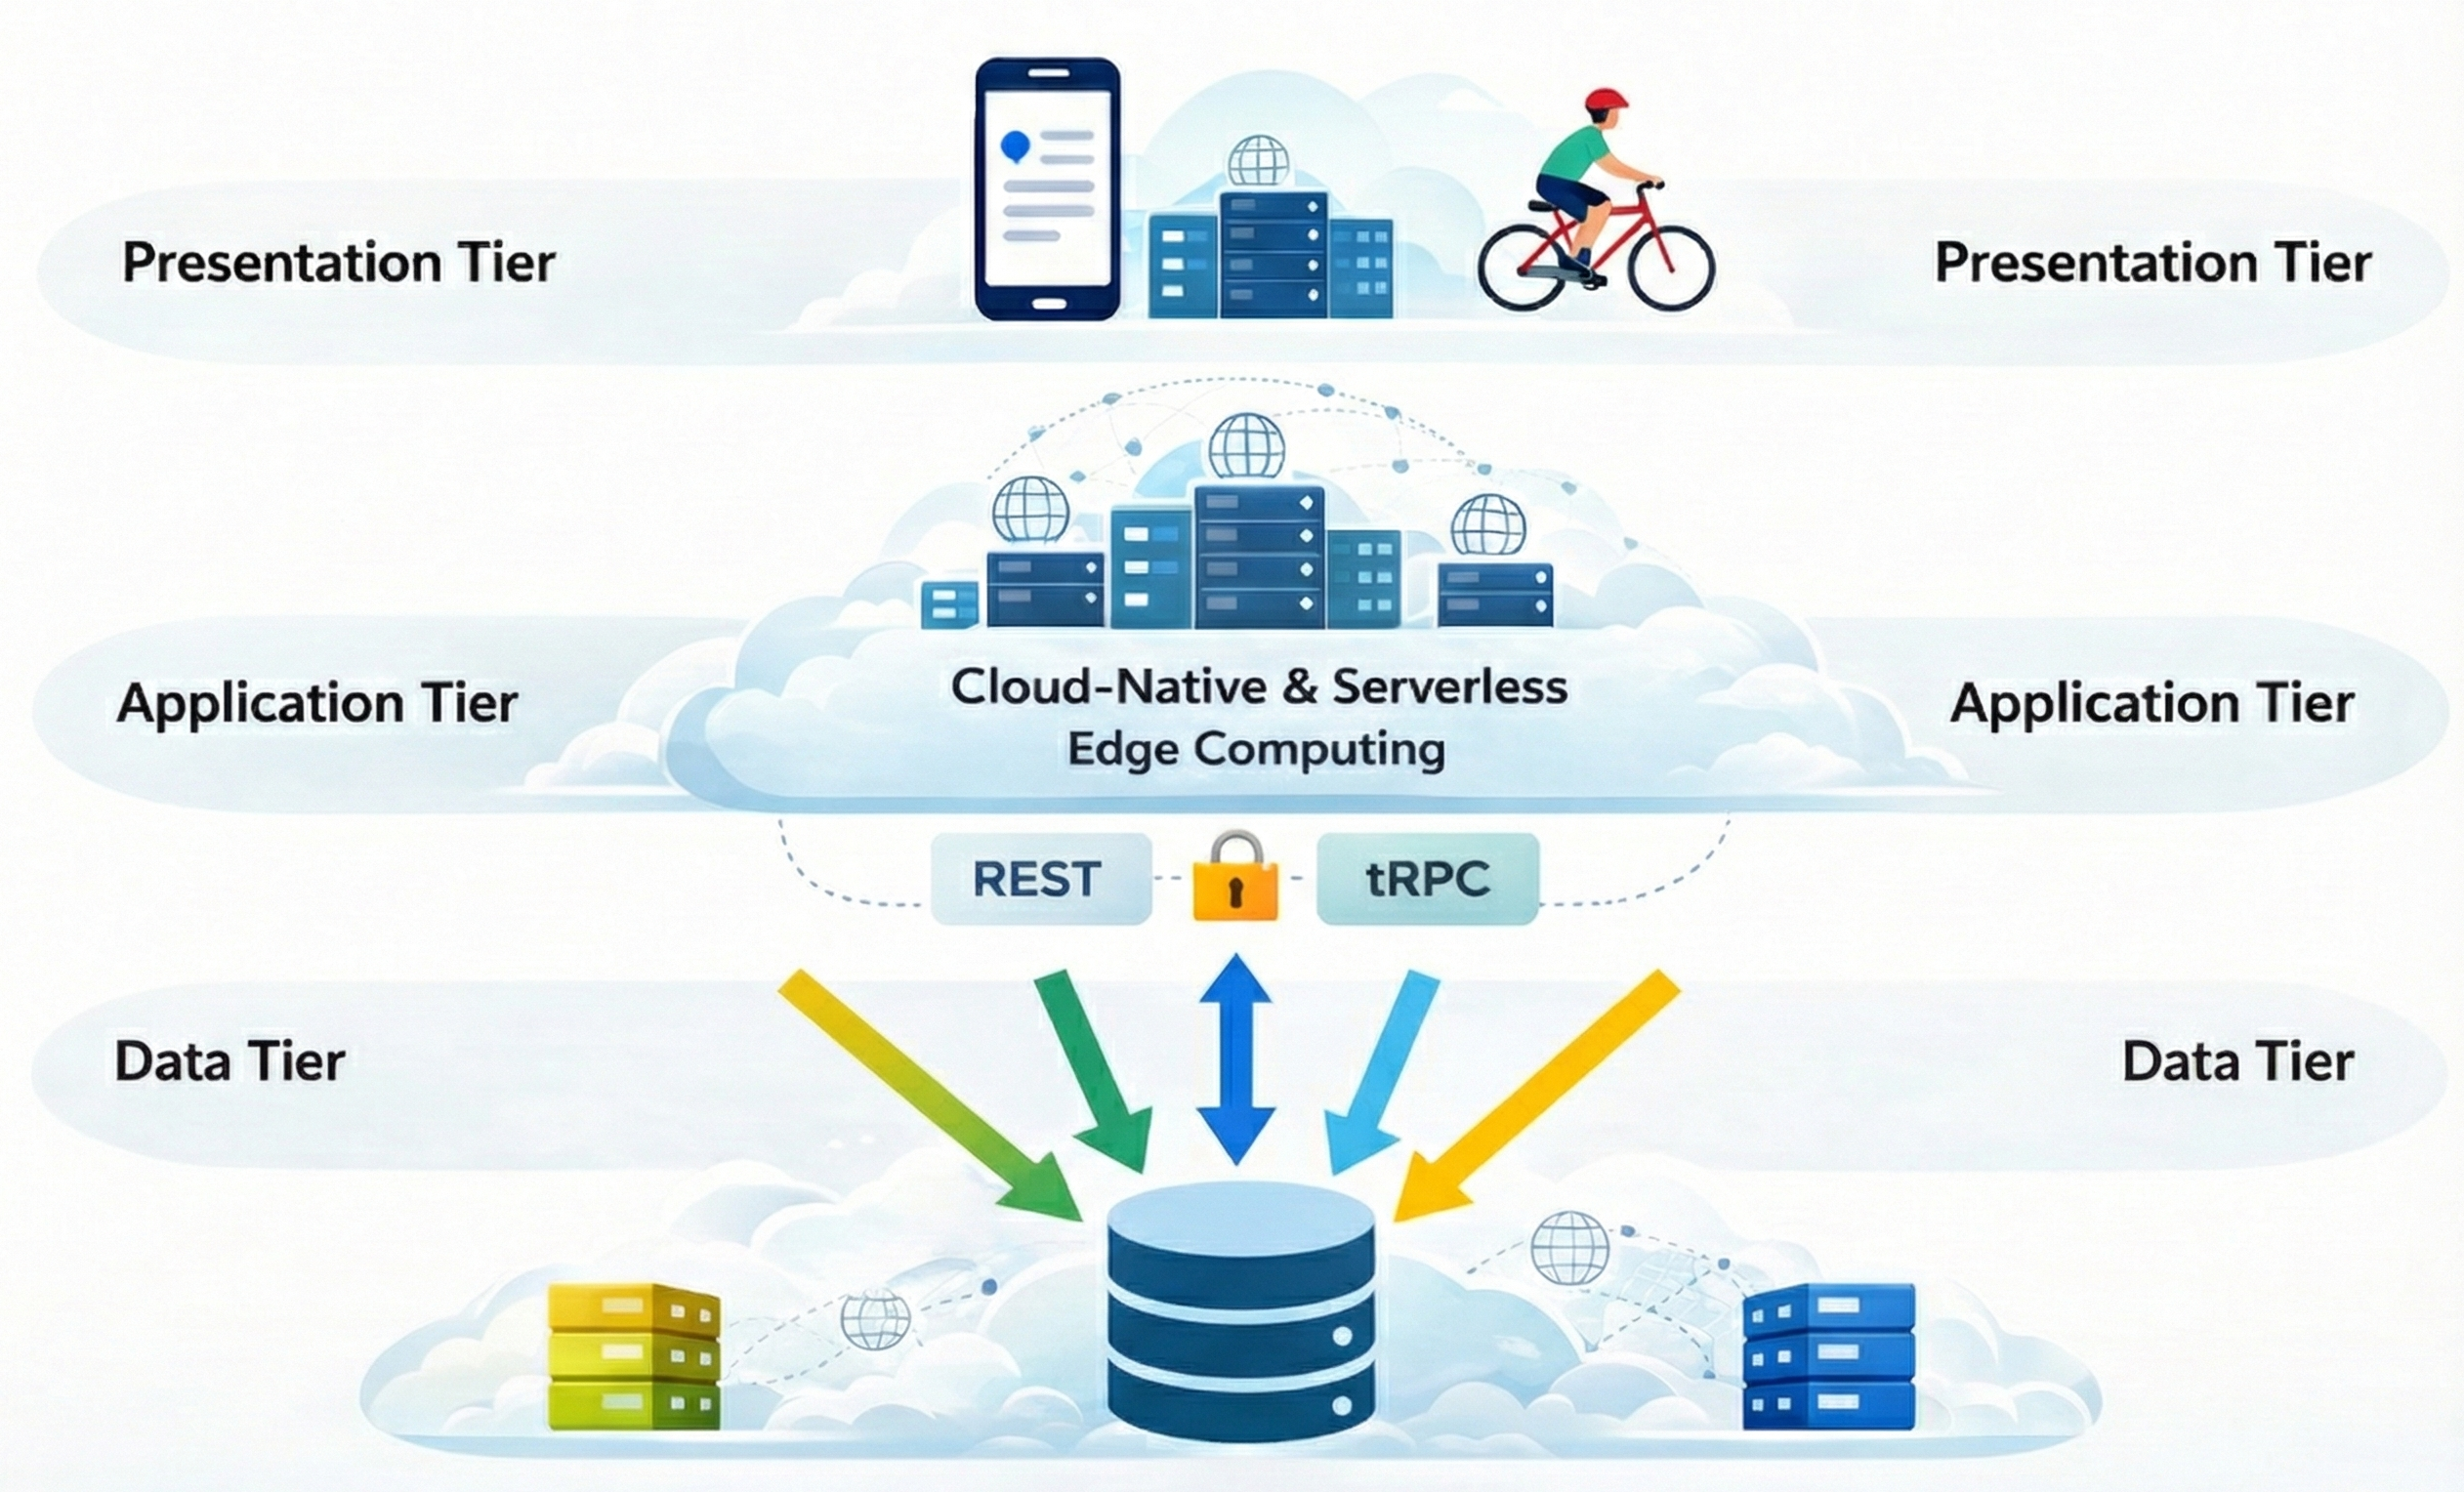
\includegraphics[width=\textwidth]{Images/2.1_SystemView.png}
\end{figure}

A defining architectural choice is the adoption of strongly typed Remote Procedure Calls (RPC) for client-server communication, implemented via tRPC. This approach establishes a strict, schema-based contract between the frontend and the backend. By sharing type definitions across the entire stack, the architecture ensures rigorous interface consistency, robust data validation, and a streamlined development workflow.

This design guarantees modularity and maintainability while supporting advanced client-side capabilities, such as sensor simulation and local state management, effectively distributing the computational load between the user device and the edge infrastructure.future new features.

% \subsection{Detailed View}

\textbf{Presentation Tier}

The user interface is not merely a passive display layer but is implemented as a “Smart Client” using a Single Page Application approach built with React. This component acts as a comprehensive runtime environment within the user's browser, taking on responsibilities that go far beyond simple visualization. Specifically, the presentation tier is designed to handle complex logic such as the local simulation of hardware sensors, generating synthetic GPS and accelerometer telemetry to demonstrate automated reporting features directly on desktop environments. 

Furthermore, the client actively manages local state and performs rigorous preliminary data validation using strict schemas shared with the backend. This active role significantly reduces the need for constant server round-trips and ensures that the user experience remains fluid and responsive even during complex interactions.

\textbf{Application Tier}

The backend architecture represents a significant departure from traditional monolithic application servers, as it is hosted entirely on a global Edge Computing infrastructure provided by Cloudflare Workers. This serverless design allows the business logic to be executed physically closer to the user, drastically reducing latency and ensuring automatic scalability during high-traffic periods without the need for manual infrastructure management. 

The core logic is organized into distinct functional modules exposed via tRPC routers, which implement a Service Layer pattern to orchestrate complex operations such as route calculation, authentication verification, and the aggregation of community data. This tier also acts as a secure gateway that mediates all interactions with external third-party services, such as OSRM for routing and weather APIs, encapsulating API keys and connection details to protect sensitive credentials from being exposed to the client.

%The backend orchestrates business logic through distinct service modules, each handling specific domain responsibilities. 

% The Trip Manager processes user-recorded routes, calculating statistics and managing trip lifecycle from creation through publication. 

% The Path Manager aggregates community-contributed routes, computing relevance scores based on crowdsourced feedback and maintaining path-to-street relationships. 

% The Obstacle Manager validates and tracks reported hazards, implementing a verification workflow where automated detections transition through user confirmation states. 

% The Authorization Manager handles authentication and session management, ensuring all API requests carry validated user context. 

% External service integrations extend platform capabilities through dedicated integration components. 

% The Routing Service interfaces with external routing engines to calculate distances and generate route geometries between waypoints. 

% The Street Service queries maps databases to retrieve actual street geometries for manual path construction. 

% The Weather Service provides environmental context for trip recordings. These integration services abstract external dependencies, allowing the core business logic to remain independent of specific provider implementations. 

% The API Gateway routes incoming requests to appropriate service modules based on operation type. Services coordinate through data access objects that encapsulate database interactions, maintaining separation between business logic and persistence concerns. This architecture supports horizontal scaling through stateless service design and vertical scaling through database connection pooling strategies.

\textbf{Data Tier}

Persistent storage employs a relational database managing structured data through schema-defined tables and relationships. The data model reflects domain entities with precision: trips capture route geometries and performance metrics; streets represent cyclable segments with condition status; paths aggregate streets into published routes discoverable by the community. 

User-generated content flows through a validation pipeline where manual reports and automated sensor detections converge into aggregated condition scores, influencing path rankings in search results. Data integrity mechanisms ensure consistency across related entities. Publishing a trip as a community path triggers the creation of path segment records linking the path to constituent streets, maintaining referential relationships. 

Deletion operations cascade through dependent records, preventing orphaned data. The schema accommodates both structured relational data for core entities and semi-structured data for variable-content fields like sensor readings and weather conditions, stored as JSON within appropriate columns. The database design supports concurrent operations through transaction isolation and optimistic locking strategies. Read-heavy operations for path discovery leverage indexing on frequently queried fields, while write operations for trip recording and reporting maintain ACID guarantees. This foundation enables reliable service delivery under varying load conditions, from individual users recording trips to community-wide path browsing during peak usage periods.

\begin{figure}[H]
    \centering
    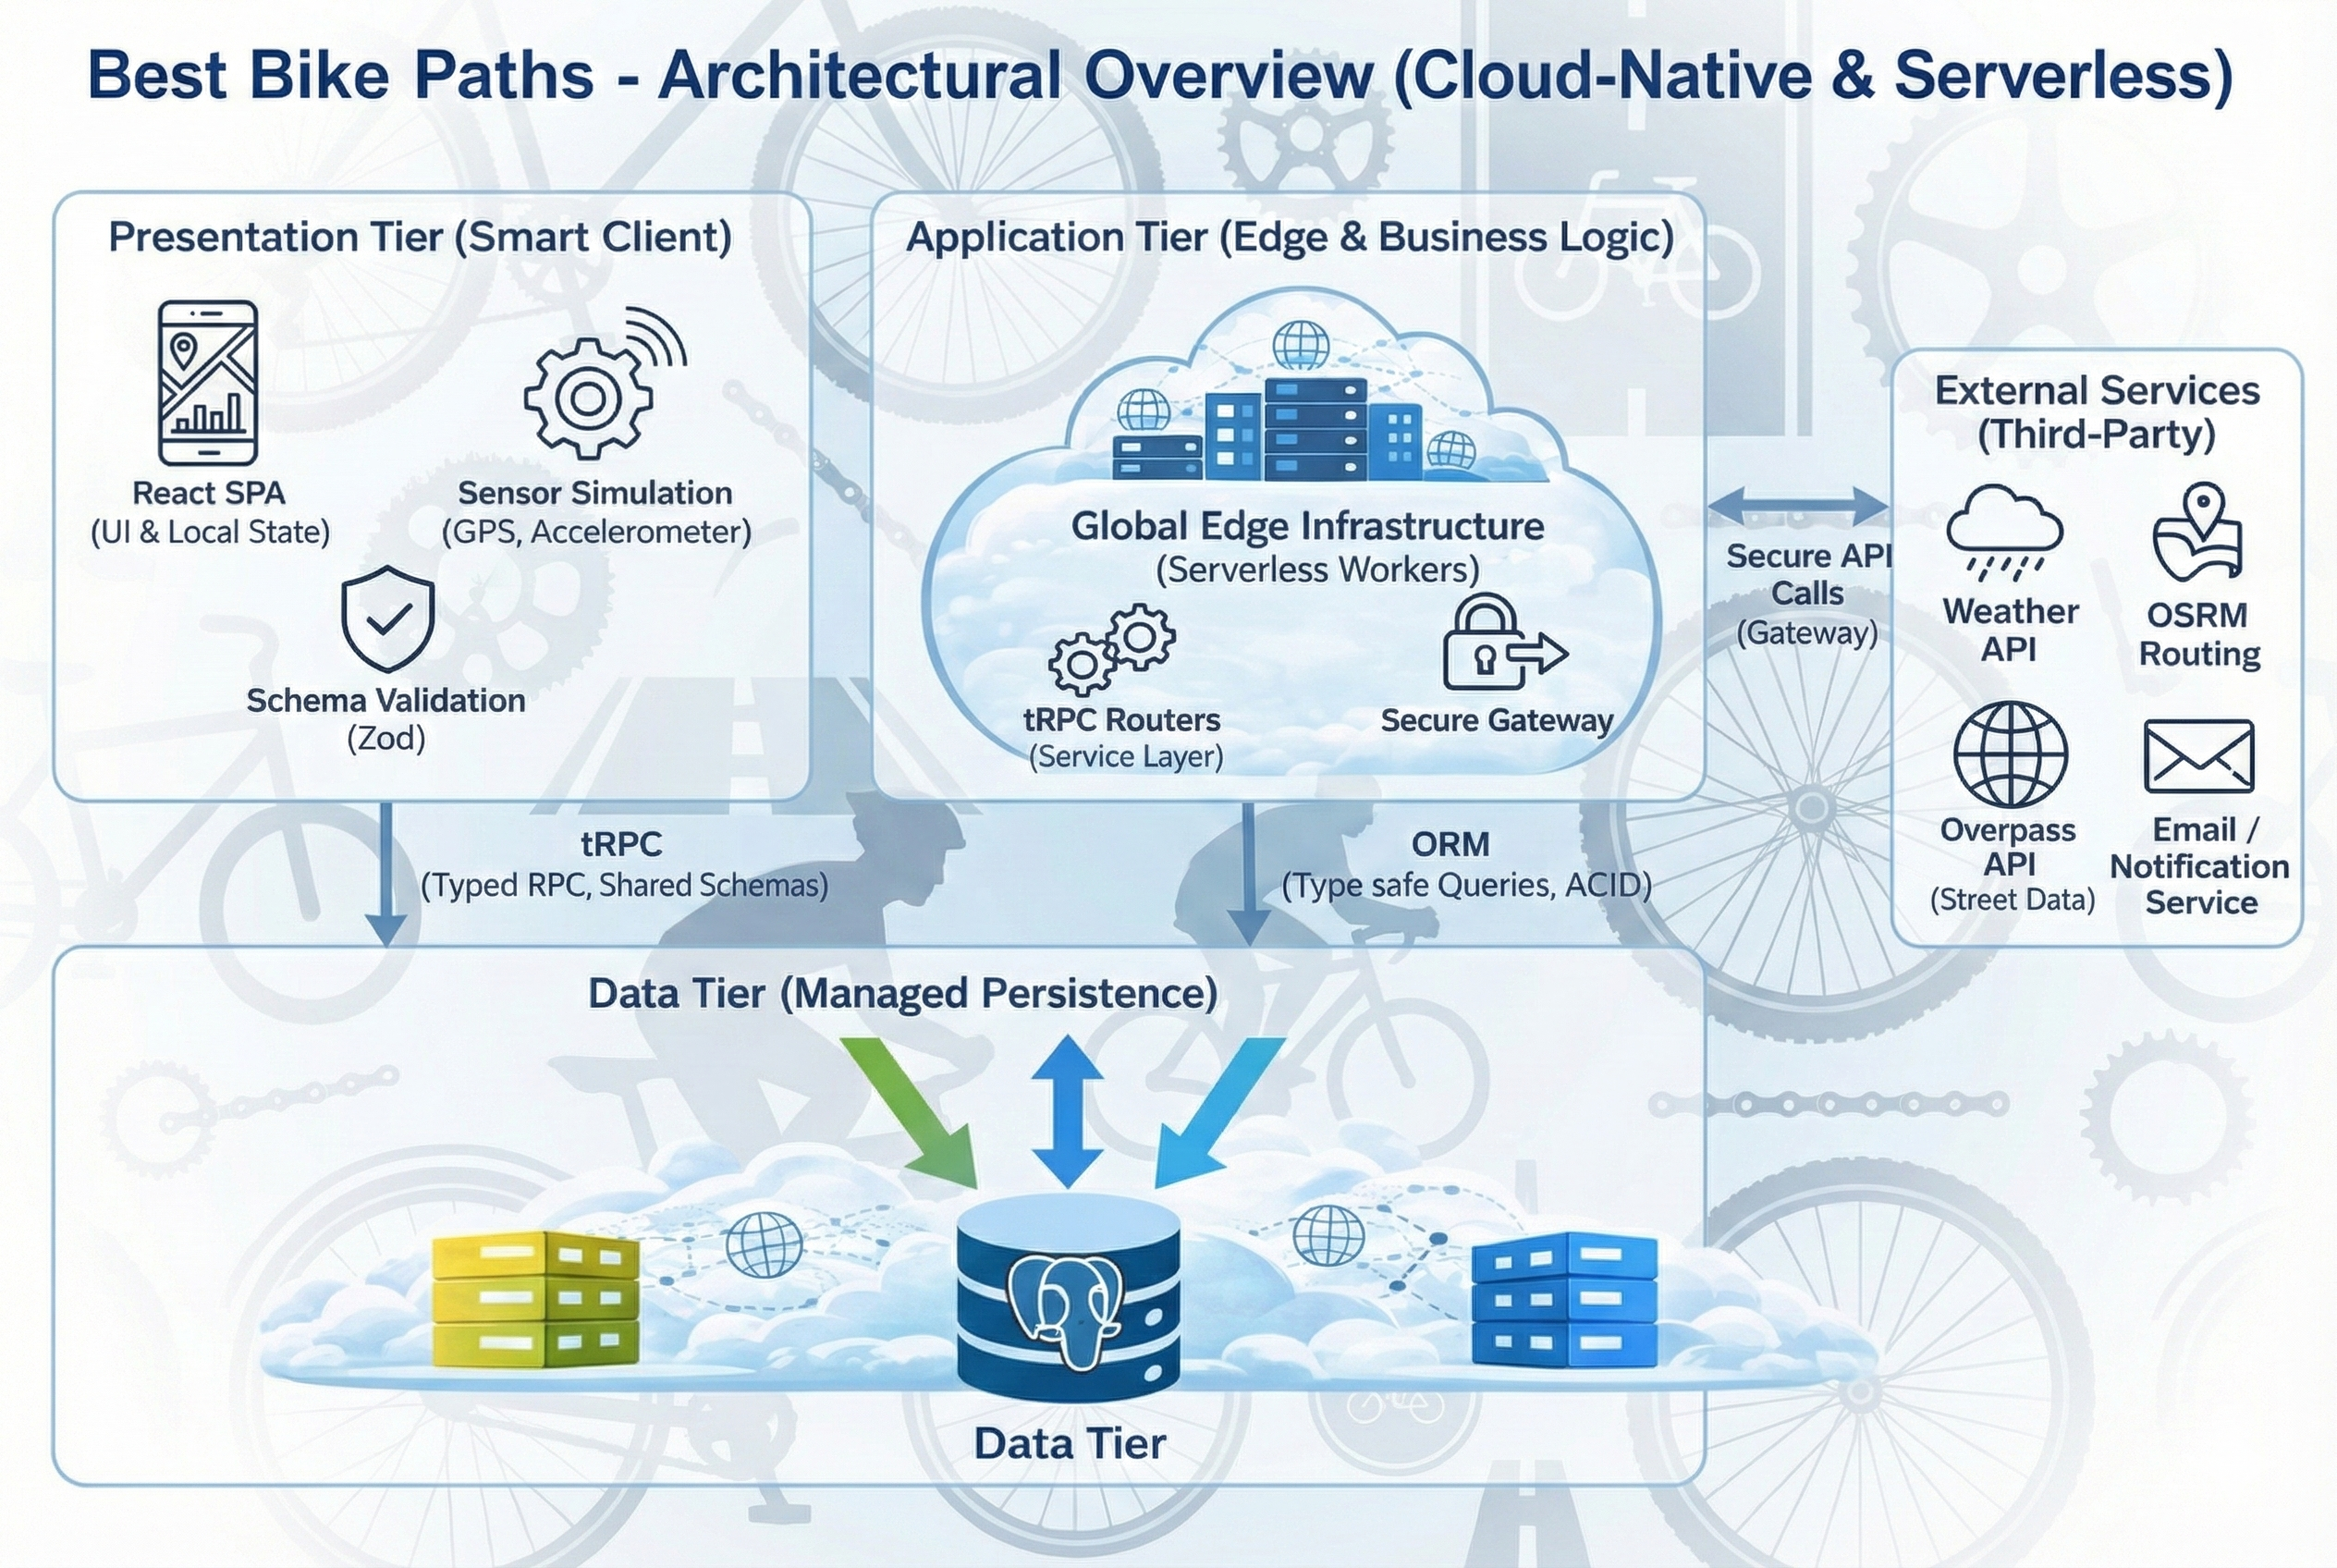
\includegraphics[width=\textwidth]{Images/2AOverview.png}
\end{figure}

\textit{All client-server communication is handled through typed RPCs targeting the Application Tier, which mediates all access to the Data Tier through an ORM-based persistence layer.}

\section{Component view}
\label{Component view} %
\begin{figure}[H]
    \centering
    \includegraphics[width=1\linewidth]{Images/bbp - component diagram.drawio.png}
\end{figure}

The following sections describe the main components of the system, organized into Back-end, Front-end, and External Services.

\subsection{Back-end components}

The back-end is hosted within an application server that acts as the entry point and manages the routing of requests toward specific services.

\textbf{API Gateway}

This component acts as the single entry point for all client requests. It intercepts HTTP calls, handles the request context (including session validation), and routes the call to the appropriate Router (Service).

\textbf{Authentication Management Service}

Responsible for handling user identities, this component integrates an external library to manage authentication flows (login, logout, session handling) and maintain active sessions. It provides the application context with information about the currently authenticated user in order to authorize protected operations.

\textbf{Trip Management Service}

This service (corresponding to TripRouter) manages the lifecycle of users’ personal trips. Its responsibilities include creating and saving new trips (recording GPS tracks), managing trip simulations, editing, deleting, and retrieving details of past trips and verifying whether a trip has already been published as a public path.

\textbf{Path Management Service}

Handles the inventory of public cycling paths.
It allows users to search for existing paths, view their details, and convert personal trips (Trip) into public cycling paths (Path).
It also supports manual creation of paths by defining a sequence of streets.

\textbf{Routing Service}

Provides route calculation functionalities.
It interacts with the external routing engine to compute the optimal route between two coordinates or across a series of waypoints (streets or addresses).
It includes the logic to validate coordinates and compute geospatial distances.

\textbf{Street Service}

This component aggregates the functionalities for managing reports (PathReportRouter and StreetRouter). It collects manual or sensor-based road condition reports, associates reports with specific streets or path segments and allows users to view and manage their own submitted reports.

\textbf{External Integration Services (Weather and Geocoding)}

A set of utility modules providing adapters to third-party APIs:
\begin{itemize}
    \item \textbf{Weather Service: }Enriches trip data with weather information retrieved according to timestamp and coordinates.
    \item \textbf{Geocoding Service: }Manages translation between textual addresses and geographic coordinates, implementing caching logic to optimize performance.
\end{itemize}

\textbf{Database Management Service (DBMS)}

Represents the data persistence layer.
The system uses a relational database (PostgreSQL) accessed through an Object-Relational Mapper (ORM).
It manages structured entities and complex geospatial data (GeoJSON) for route and position storage.

\subsection{Front-end Components}

The client is a responsive web application (React) designed to deliver a smooth user experience similar to a native app.

\textbf{Web App and Router}

Main container that handles the application lifecycle and client-side navigation.
It manages the page structure, dynamic routing, and protection barriers for user-restricted areas.

\textbf{State Management and Caching Layer}

A cross-cutting layer for data management:
\begin{itemize}
    \item Server State: Manages cached data coming from APIs to optimize performance and reduce network calls.
    \item Client State: Manages local and volatile UI state.
\end{itemize}

\textbf{Map Visualizer}

Core graphical component responsible for geospatial rendering.
It displays saved paths (GeoJSON), selected streets, and points of interest.
It offers interactive functionalities such as zooming, panning, and coordinate selection on the map to define origins and destinations.

\textbf{Trip Recorder}

Module managing trip acquisition logic.
In Automated mode, since the app runs in a browser, this component software simulates the behavior of physical sensors (GPS, accelerometer), generating synthetic GPX tracks and sending simulated telemetry data to the back-end.
It displays real-time statistics of the ongoing trip.

\textbf{Path Reporting Builder}

Interface dedicated to manual data entry (ManualPathBuilder).
It allows the user to compose a path by selecting a sequence of streets or map points and completing detailed forms to report road surface conditions or the presence of obstacles.

\textbf{Route Discovery}

Search and navigation interface (RouteFinder).
It enables users to input search criteria (origin/destination), view route options computed by the server ordered by Score, and consult details of available public paths.

% \subsection{External Services}

% The BBP system depends on the following external services to complete its functionalities:

% \textbf{Open Source Routing Machine (OSRM):} Used by the back-end to compute the geometry of cycling paths and travel distances.

% \textbf{OpenStreetMap:} Used for Geocoding services (street and address lookup).

% \textbf{Map Tile Provider:} Service supplying base map tiles displayed in the front-end.

\section{Deployment view}

This chapter presents the Deployment View of the Best Bike Paths platform, which is graphically represented in the figure below. This view aims to describe the execution environment of the system, detailing the physical and logical distribution of the hardware components and cloud services that support the application software.  
Unlike traditional architectures based on centralized monolithic servers, BBP adopts a modern Cloud-Native and Serverless architectural approach. This design choice allows the management of the underlying infrastructure to be delegated to specialized providers, while ensuring high availability, automatic scalability, and reduced global latency through the use of Edge Computing technologies.

\begin{figure}[H]
    \centering
    \includegraphics[width=0.8\linewidth]{Images/bbp - deployment diagram.drawio.png}
\end{figure}


The following section provides additional details concerning the elements shown in the deployment diagram, analyzing the role of each node and the interactions that occur among them.

\textbf{User Device}

This node represents the physical terminal used by the end user to interact with the system, which may be a personal computer, a smartphone, or a tablet. The fundamental software requirement for this node is the presence of a modern web browser. When a user accesses the platform’s URL, the device does not simply display static pages but downloads and executes the entire Single Page Application (SPA) developed in React. Consequently, the browser acts as a true runtime environment for the presentation logic: it handles the rendering of the user interface, local state management, and preliminary form validation.  
In the specific context of the BBP demo, this node also plays a critical role in sensor simulation: the JavaScript code running on the client simulates the behavior of GPS and accelerometer sensors (normally present on mobile hardware) to generate telemetry data required for the “Automated Reporting” functionality. All outgoing communications from this node to the system occur over the secure HTTPS protocol.


\textbf{Cloudflare Edge  }

This node constitutes the core of the backend infrastructure. Instead of residing on a single physical server located in a specific geographic area, the application is deployed on Cloudflare’s global Edge Network. Two logical subcomponents can be identified within this environment: 
\begin{itemize}
    \item Component Pages that acts as a Content Delivery Network (CDN). Its purpose is to host the static assets of the application (HTML files, CSS stylesheets, and compiled JavaScript bundles) and serve them to users from the geographically closest server, drastically reducing initial loading times.  
    \item Component Workers that hosts the actual API Server. Here, the Hono framework and the tRPC routers responsible for the business logic are executed. Whenever the user’s device sends a data request (for example, to save a route or perform login), it is intercepted and processed by an ephemeral “serverless” instance. This approach ensures that computing resources are dynamically allocated only when needed, handling traffic spikes without manual intervention.
\end{itemize}

\textbf{PostgreSQL (Database)}

This node represents the data persistence layer (Data Tier). To guarantee the integrity and security of information, the database is decoupled from the application layer and hosted on a managed cloud service. It is a PostgreSQL instance optimized for the cloud, responsible for storing all domain entities: user profiles, authentication sessions, road condition reports, and, most importantly, complex geospatial data (GeoJSON) related to cycling routes.  
The application running on Cloudflare Edge communicates with this database node via a secure SSL-encrypted TCP connection, using a connection pool optimized for serverless environments. This separation ensures that data remains persistent and protected regardless of the lifecycle of the application processes.

\textbf{External Services}  

The BBP system does not operate in isolation but integrates with an ecosystem of third-party services to provide advanced functionality without the need to reimplement complex solutions from scratch.  
\begin{itemize}
    \item OSRM (Open Source Routing Machine): The public routing engine queried by the backend to compute optimal cycling routes between two points and to perform the map-matching of raw GPS traces.  
    \item Overpass: A service based on OpenStreetMap used for geocoding operations, i.e., translating textual addresses into geographic coordinates and vice versa.  
    \item OpenWeather: An external weather API consulted to enrich saved trip data with the atmospheric conditions (temperature, wind, and weather) recorded at the time of the activity. It is important to note that, for security and architectural reasons, it is always the Cloudflare Edge node that interacts with these external services, acting as an intermediary for the client. This pattern hides the complexity of third-party APIs from the user’s device and protects any private access keys.
\end{itemize}

\newpage
\section{Runtime View}

\textbf{Signup Cyclist}

\begin{figure}[H]
    \centering
    \includegraphics[width=1\linewidth]{Images/bbp - signup.png}
\end{figure}
User submits the registration form in the browser, which is sent to ‘/api/auth/register’ and forwarded to the Authorization Manager. The manager validates the input and checks via ‘UserDAO.checkEmailExists(email)’ whether the email is already in the database.

If the email exists, it returns an error response 422. If not, it hashes the password, creates the user via ‘UserDAO.createUser(...)’, creates a session via ‘createSession(userId)’, and returns success 200 with a session token so the user is registered and logged in.

\newpage
\textbf{Signin Cyclist}
\begin{figure}[H]
    \centering
    \includegraphics[width=1\linewidth]{Images/bbp - signin.png}
\end{figure}
User submits login credentials to ‘/api/auth/login’, which the User Interface forwards to the Authorization Manager. The manager validates the input, fetches the user by email via ‘UserDAO.findUserByEmail(email)’, and returns 401 if the user doesn’t exist.

If the user exists, it verifies the password against the stored hash; on failure it returns 401. On success, it creates a session via ‘createSession(userId)’ (stored by the DAO), returns 200 with a session token, and the user is logged in.

\newpage
\textbf{Paths Lookup}
\begin{figure}[H]
    \centering
    \includegraphics[width=1\linewidth]{Images/bbp - path lookup.png}
\end{figure}
The browser calls ‘/api/paths/search’, and the User Interface forwards the request to the Path Manager, which asks the PathDAO for the most relevant paths from the database. For each returned path, the Path Manager fills in missing route geometry by computing it from the underlying street segments and, when trip data is present, also loads any recorded obstacles for that path. It then returns the completed path collection with status code 200 (OK), which indicates the request succeeded, and the UI renders the paths and condition information on the interactive map.

\newpage
\textbf{Record manually a trip}
\begin{figure}[H]
    \centering
    \includegraphics[width=1\linewidth]{Images/bbp - manual recording diagram.png}
\end{figure}
On the trip recording page, the user enters basic trip details and searches for a street, and the Street Service uses the Overpass API to fetch the selected OpenStreetMap street geometry so it can be shown on the map. After the user clicks start and end points on that geometry, the UI calls the Routing Service, which queries OSRM to compute a real cycling route between the two coordinates and returns route distance and geometry rather than a straight-line estimate. The user can repeat this to build a multi-segment trip, optionally mark obstacles on the map, then submit the trip so the backend stores the trip, its routes, and its obstacles in the database and returns a success response.

\newpage
\textbf{Record automatically a trip}
\begin{figure}[H]
    \centering
    \includegraphics[width=1\linewidth]{Images/bbp - automated recording.png}
\end{figure}

The user opens the trip recording page, switches on Automatic Mode, and the User Interface hands trip generation to a Trip Simulator that creates a simulated ride by generating multiple route segments from random coordinate pairs. For each segment, the simulator calls the Routing Service, which queries OSRM to return realistic routing results such as route distance, duration, and route geometry, so the simulated trip still follows the street network.  The simulator then generates plausible weather values, places obstacles by sampling points along the computed route geometry, totals the trip duration by summing segment durations, and sets a default rating before showing everything in a summary modal for confirmation. After the user confirms (“Keep These Routes”), the Trip Manager persists the trip as “simulated” (including weather JSON), saves each route and obstacle, marks obstacles as “automated,” and returns a success response to notify the user that the simulated trip was recorded.

\newpage
\textbf{Verify detected obstacles}
\begin{figure}[H]
    \centering
    \includegraphics[width=1\linewidth]{Images/bbp - verify obstacles.png}
\end{figure}

The user navigates to the trip detail page where the User Interface requests all obstacles associated with the trip from the Obstacle Manager. The system retrieves obstacles from the database and displays them with their current status: PENDING (awaiting verification), CONFIRMED (verified), REJECTED (false positive), or CORRECTED (updated details). When the user updates an obstacle status—whether confirming its existence, rejecting it as a false positive, or correcting its details—the system follows a unified workflow. The Obstacle Manager first verifies that the authenticated user owns the obstacle by querying the database. If ownership verification fails, a 403 Unauthorized error is returned. If successful, the system updates the obstacle record with the new status and any associated data modifications (such as corrected coordinates or descriptions), then returns a success response.

\newpage
\textbf{Paths Browsing}
\begin{figure}[H]
    \centering
    \includegraphics[width=1\linewidth]{Images/bbp - path browsing.png}
\end{figure}

The user navigates to their personal paths area where the User Interface requests all trips belonging to the authenticated user from the Trip Manager. The system queries the database and displays the user's trip collection with statistics. When publishing a trip to the community, the user provides a path name and initiates the publication. The Trip Manager validates the trip by checking that a rating exists and all obstacles have been verified. If validation fails due to missing rating or pending obstacles, a 400 Bad Request error is returned prompting the user to complete these requirements. If validation passes, the Path Manager creates a public path record in the database, links it to the trip's street segments through path\_segment records, and marks the trip as published. For trip deletion, the system verifies user ownership and executes the delete operation, which cascades to remove all associated routes and obstacles through database foreign key constraints.

\section{Component Interfaces}

\subsection{HTTP endpoints}
These are direct HTTP routes accessible via standard HTTP methods:

\textbf{System Information}
\begin{itemize}
    \item GET /api - Returns API metadata and available endpoints
    \item GET /health - Health check endpoint returning system status
\end{itemize}

\textbf{OSRM Routing Proxy}
\begin{itemize}
    \item GET /api/osrm/route/:profile/:coordinates - Proxies routing requests to Open Source Routing Machine
\end{itemize}

\textbf{Authentication (Better Auth)}
\begin{itemize}
    \item GET /api/auth/* - Authentication endpoints (login, signup, session management)
    \item POST /api/auth/* - Authentication mutations (handled by Better Auth library)
\end{itemize}

\textbf{Authentication (Better Auth)}
\begin{itemize}
    \item GET /api/auth/* - Authentication endpoints (login, signup, session management)
    \item POST /api/auth/* - Authentication mutations (handled by Better Auth library)
\end{itemize}

\subsection{tRPC API Procedures}
All tRPC procedures are accessible via /api/trpc endpoint with batching support enabled.

\textbf{User Router (user.*)}
User profile and account management.
\begin{itemize}
    \item get\_me() - Returns current authenticated user profile
    \item put\_updateProfile(name?) - Updates user profile information
\end{itemize}

\textbf{Trip Router (trips.*)}
Bike trip recording, route management, and obstacle reporting.

\textit{Trip Management}
\begin{itemize}
    \item post\_create(name, description?, startTime, endTime, collectionMode, distance?, avgSpeed?, duration?, weatherData?) - Creates a new trip
    \item get\_list() - Lists all trips for the current user, ordered by creation date
    \item get\_detail(tripId) - Gets trip details with all routes ordered by routeIndex
    \item get\_isPublished(tripId) - Checks if a trip has been published as a community path
    \item put\_updateTripStats(tripId, distance?, avgSpeed?, duration?) - Updates trip statistics from route data
    \item post\_delete(tripId) - Deletes a trip and all associated routes, obstacles, and path records
\end{itemize}

\textit{Route Management}
\begin{itemize}
    \item post\_addRoute(tripId, name, geometry, distance, startLat, startLon, endLat, endLon) - Adds a route segment to a trip
    \item post\_removeRoute(tripId, routeIndex) - Removes a route and reindexes remaining routes
    \item post\_reorderRoutes(tripId, newOrder) - Reorders routes within a trip
    \item post\_simulate(tripId, numRoutes?) - Generates simulated routes for testing (default: 5 routes)
\end{itemize}

\textit{Rating System}
\begin{itemize}
    \item post\_addRating(tripId, rating, notes?) - Adds or updates trip rating (1-5 scale, required before publishing per RASD)
    \item get\_getRating(tripId) - Retrieves trip rating if exists
\end{itemize}

\textit{Obstacle Reporting}
\begin{itemize}
    \item post\_addObstacle(tripRouteId, type, description?, lat, lon, detectionMode, sensorData?, status?) - Reports an obstacle on a trip route
    \item get\_getObstacles(tripId) - Lists all obstacles for a trip with route context
    \item put\_updateObstacleStatus(obstacleId, status, description?, lat?, lon?) - Updates obstacle lifecycle status (confirm/reject/correct per RASD)
\end{itemize}

\textit{Publishing}
\begin{itemize}
    \item post\_publish(tripId, pathName, pathDescription?) - Publishes trip as a public community path (requires rating, per RASD)
\end{itemize}

\textbf{Path Router (path.*)}
Community path discovery, creation, and reporting.

\textit{Path Discovery}
\begin{itemize}
    \item get\_search(query?, limit?) - Searches for paths by name, ordered by score (public, limit: 1-50, default: 20)
    \item get\_getDetails(id) - Gets path details with constituent streets and obstacles (public)
    \item get\_getPathStreets(pathId) - Lists streets composing a path in order (public)
\end{itemize}

\textit{Path Creation}
\begin{itemize}
    \item post\_upsertPath(name, description?, geometry) - Creates or retrieves path by geometry (protected)
    \item post\_createManualPath(name, description?, streetIds, geometry?) - Creates path from ordered street list (geometry computed from streets)
    \item post\_publishTripAsPath(tripId, pathName?) - Converts private trip to public path with street linking
    \item Path Reporting
    \item post\_submitReport(pathId, rating?, streetReports, obstacles?) - Submits condition report for path streets
    \item streetReports: Array of {streetId, status}
    \item obstacles: Array of {type, description, lat, lon}
\end{itemize}

\textbf{Path Report Router (pathReport.*)}
Crowdsourced condition reporting for trip routes and streets.

\textit{Report Management}
\begin{itemize}
    \item post\_create(tripRouteId?, streetName?, lat?, lon?, status, obstacles?, isPublishable?, collectionMode?, rating?) - Creates new report (trip-based or standalone street report)
    \item get\_list(status?, limit?, offset?) - Lists published reports with pagination (public, limit: 1-100, default: 50)
    \item get\_detail(reportId) - Gets report detail with route, trip, and user context (public, only publishable reports)
    \item put\_update(reportId, status?, obstacles?, isPublishable?, isConfirmed?) - Updates report properties
    \item post\_delete(reportId) - Deletes user's own report
    \item get\_myReports() - Lists current user's reports including drafts
\end{itemize}

\textbf{Street Router (street.*)}
Street discovery, search, and condition reporting.

\textit{Street Discovery}
\begin{itemize}
    \item get\_getDetails(id) - Gets street details with recent reports (last 30 days, public)
    \item get\_list(cyclableOnly?, city?, limit?) - Lists streets with filters (public, limit: 1-100, default: 50, cyclableOnly: default true)
\end{itemize}
\textit{Street Reporting}
\begin{itemize}
    \item post\_createReport(streetId, status, collectionMode, obstacles?, sensorData?, isPublishable?, isConfirmed?) - Creates condition report for street
    \item get\_myReports(limit?) - Lists user's street reports (limit: 1-50, default: 20)
\end{itemize}

\textbf{Routing Router (routing.*)}
Route finding and navigation between locations.

\begin{itemize}
    \item get\_findRoutes(startStreetName, endStreetName) - Finds routes between two streets using existing path data (public)
    \item get\_getRouteDetails(routeId) - Gets detailed route information with streets and recent reports (public)
\end{itemize}


\section{Selected architectural styles and patterns}

The design of Best Bike Paths (BBP) is not limited to simple functional implementation but adopts established architectural styles and specific design patterns to ensure modularity, maintainability, and a clear separation of responsibilities. The following sections analyze the main structural choices adopted.

\subsection{Architectural Styles}

Layered Architecture (N-Tier) To guarantee a clear separation of concerns, the system's back-end has been structured according to the Layered Architecture style. This organization provides for a unidirectional and hierarchical data flow, where each layer depends exclusively on the one below it, remaining agnostic to the implementation details of the layer above. Specifically, the architecture is divided into four logical layers:

\begin{itemize}
    \item \textbf{Presentation Layer:} Managed by the Hono framework and tRPC procedures, this layer is responsible for exposing API endpoints, validating incoming inputs, and handling the serialization of responses sent to the client.
    \item \textbf{Business Logic Layer:} Composed of “Services” (or logical Routers), this layer encapsulates the application's domain rules, such as calculating path scores or managing user sessions.
    \item \textbf{Data Access Layer:} This layer abstracts the interaction with the relational database. Thanks to the use of Drizzle ORM, SQL queries are encapsulated within type-safe methods, protecting the business logic from the complexity of the underlying query language.
    \item \textbf{External Integration Layer:} A layer dedicated to interacting with third-party services (OSRM, Nominatim, OpenWeather), acting as an adapter to normalize external data before it enters the system.
\end{itemize}

\textbf{Client-Server with RPC (Remote Procedure Call)}

Unlike the classic RESTful style, BBP adopts an approach based on strongly typed RPC (Remote Procedure Call), implemented via the tRPC library. In this model, the client does not invoke generic resources via HTTP verbs, but directly calls “procedures” defined on the server (e.g., trip.create, path.getBest). This architectural choice was dictated by the need to maintain strict consistency between the Frontend (React) and the Backend. Since both share TypeScript type definitions, the system ensures that any modification to a function signature on the server is immediately detected as a compilation error on the client, drastically increasing Reliability and development speed.

\textbf{Component-Based Architecture (Frontend)}

The user interface strictly follows a component-based architecture. The application is not a monolithic block of HTML and JavaScript but is composed of independent, reusable, and encapsulated units (React Components). This style allows the presentation logic of each element (such as a path card or a reporting form) to be isolated, making the system easily extensible. The adoption of this architecture is supported by the Compound Components pattern (used in the shadcn/ui library), which allows for the construction of complex interfaces by assembling primitive components in a flexible manner, improving the readability and maintainability of the source code.

\subsection{Backend Design Patterns}

\textbf{Service Layer Pattern}

To prevent business logic from residing within HTTP request handlers (or tRPC procedures), a Service Layer was introduced. Specific classes or modules, such as the RoutingService, contain the pure application logic. For example, the mathematical calculation to aggregate user reports and determine the condition of a street does not occur at the API entry point but is delegated to the aggregation service. This pattern fosters code reuse and simplifies unit testing, as services can be tested independently of the web infrastructure.

\textbf{Strategy Pattern}

The requirement to support different modes of trip data acquisition (manual entry, simulated automated detection, or pure routing) was resolved by implementing the Strategy Pattern. The system defines a common interface for creating a “Trip” but the concrete algorithm varies based on the collectionMode parameter.

\begin{itemize}
    \item In the “Manual” case, the strategy is limited to saving the data entered by the user.
    \item In the “Simulated” case, the strategy invokes the synthetic track generator.
    \item In the “OSRM” case, the strategy consults the external routing service. This allows for the addition of new acquisition modes in the future without modifying the existing code that handles trip saving.
\end{itemize}

\textbf{Middleware Pattern}

Cross-cutting request management is entrusted to a chain of Middleware. Before a request reaches the business logic, it passes through a series of intermediate functions responsible for injecting necessary dependencies. One middleware injects the database instance (db), another handles authentication by injecting the user object (auth), and yet another handles logging. This approach centralizes the management of cross-cutting concerns such as security and configuration, avoiding code duplication in every single procedure.

\subsection{Frontend Design Patterns}

\textbf{Container/Presentational Pattern}

In the frontend, the decision was made to separate data retrieval logic from visualization logic. “Container” components (often coinciding with Navigation Routes, e.g., TripsPage) are responsible for interacting with APIs and managing loading states and errors. Once the data is obtained, it is passed via props to “Presentational” components (e.g., TripList), which are pure and solely responsible for how information is displayed on the screen. This separation improves the testability of graphical components and the clarity of the data flow.

\textbf{Segregated State Management}

Application state management is not monolithic but clearly distinguishes between Server State and Client State.

\begin{itemize}
    \item For data originating from the server (e.g., trip lists, weather details), a Data Fetching/Caching pattern is used (via TanStack Query). This automatically handles cache validity, background refetching, and request deduplication.
    \item For volatile interface state (e.g., active search filters, unsubmitted forms), an Atomic pattern is used (via Jotai), where the state is fragmented into small independent units (“atoms”) that avoid unnecessary re-renders of the entire page.
\end{itemize}

\section{Other Design Decisions}

This section illustrates further design decisions that, while not strictly falling under classic pattern definitions, proved fundamental to satisfying the specific requirements of the BBP project.

\textbf{Monorepo with Workspaces}

The source code has been organized into a single repository (Monorepo) managed via Bun workspaces. This structure allows hosting the frontend application (/apps/app), the backend (/apps/api), and shared packages (/packages/core, /db) within the same development environment. The main motivation for this choice lies in the ability to share code and type definitions between client and server without having to publish external libraries. For instance, the database schema or utility functions for coordinate calculation are defined once and imported directly where needed, ensuring there are never mismatches between the two parts of the system.

\textbf{Schema-First API Design and Type Safety }

To ensure interface robustness, a Schema-First approach based on the Zod validation library was adopted. Instead of manually writing input control logic, each API endpoint pre-defines a strict schema of expected data. This schema is used both at runtime to validate incoming requests (automatically rejecting malformed data) and at compile-time to generate TypeScript types. This design decision creates a binding contract between frontend and backend: if the backend modifies a schema, the frontend stops compiling until it is updated, preventing a vast class of runtime bugs typical of web applications.

\textbf{Client-Side Sensor Simulation}

A critical decision for the demo development was to implement sensor simulation (GPS, accelerometer) directly in the user's browser (User Device node) rather than on the server. Since the demo application runs in a desktop web environment that lacks actual motion sensors or moving GPS, the frontend includes a simulation module (“Virtual Sensors”). This module generates synthetic GPX tracks and plausible telemetry data locally. This architectural choice allows for faithful demonstration of the “Automated Data Collection” requirement defined in the RASD without requiring dedicated mobile hardware for the testing and presentation phase, shifting the simulation complexity to the client to avoid burdening the backend with dummy data.

\textbf{Dependency Injection via Context}

To improve testability and decoupling, the backend uses a manual Dependency Injection pattern via the tRPC context. Instead of directly importing global instances (such as the database connection or Redis client) inside functions, these are injected into the request “Context” at startup. During testing, this allows the real database to be easily substituted with a mock or an in-memory database, completely isolating the unit of code under test from external infrastructures.